\section{Background}
\label{cha:background}

This chapter provides the necessary background and concepts that are applied in \ref{cha:approach} of this thesis. The sections will cover general concepts of High-Performance Computing and Scientific Workflows and will further elaborate on Monitoring, Co-location, and Machine Learning techniques applied in this work.

\subsection{High Performance Computing}
\label{sec:background_hpc}
High-Performance Computing (HPC) encompasses a collection of interrelated disciplines that together aim to maximize computational capability at the limits of current technology, methodology, and application. At its core, HPC relies on specialized electronic digital machines, commonly referred to as supercomputers, to execute a wide variety of computational problems or workloads at the highest possible speed. The process of running such workloads on supercomputers is often called supercomputing and is synonymous with HPC. The fundamental purpose of HPC is to address questions that cannot be adequately solved through theory, empiricism, or conventional commercial computing systems. The scope of problems tackled by supercomputers extends beyond traditional scientific and engineering applications to include challenges in socioeconomics, the natural sciences, large-scale data management, and machine learning. An HPC application refers both to the problem being solved and to the body of code, or ordered instructions, that define its computational solution \cite{STERLING201843}.

% Figure with architecture.
\begin{figure}[H]
    \centering
    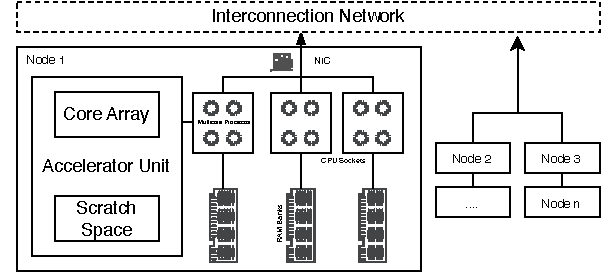
\includegraphics[scale=1.2]{fig/02/02-hpc-nodes.pdf}
    \small
    \caption{HPC Architecture}
    \label{fig:02-hpc-nodes}
    \tiny
    High-level Architecture of a HPC Data Center.
\end{figure}

Figure \ref{fig:02-hpc-nodes} shows what distinguishes HPC systems from conventional computers is their organization, interconnectivity, and scale. According to \cite{STERLING201843} scale refers to the degree of both physical and logical parallelism: the replication of essential physical components such as processors and memory banks, and the partitioning of tasks into units that can be executed simultaneously. While parallelism exists in consumer devices like laptops with multicore processors, HPC systems exploit it on a vastly larger scale, structured across multiple hierarchical levels. Their supporting software is designed to orchestrate and manage operations at this level of complexity, ensuring efficient execution across thousands of interconnected components.

\subsubsection{Modern HPC Hardware}
\label{sec:background_hpc_hardware}

High-performance computing (HPC) architecture defines how supercomputers are structured, how their components interact, and which instruction set architecture (ISA) they expose to the applications running on them. It is designed to use underlying hardware technologies efficiently to minimize time to solution, maximize computational throughput, and support large-scale, computation-intensive workloads.
The performance of an HPC system depends largely on the speed and coordination of its components, with processor clock frequency playing a central role. Modern architectures aim to balance computation, memory, and communication performance while maintaining reasonable cost, power consumption, and ease of use to achieve high application throughput.
Power consumption is a critical factor in HPC, as processors, memory, interconnects, and I/O devices all require electricity, and the resulting heat must be removed to avoid failure. Air cooling suffices for smaller systems, but high-density, high-performance systems increasingly rely on liquid cooling to achieve higher packing density and performance. Modern processors further support power management through dynamic voltage and frequency scaling, variable core activation, and thermal monitoring. These mechanisms enable a balance between power consumption and performance, guided by software that can set or adjust configurations at runtime based on workload demands \cite{STERLING201843}.

% Fig from processor
\begin{figure}[H]
    \centering
    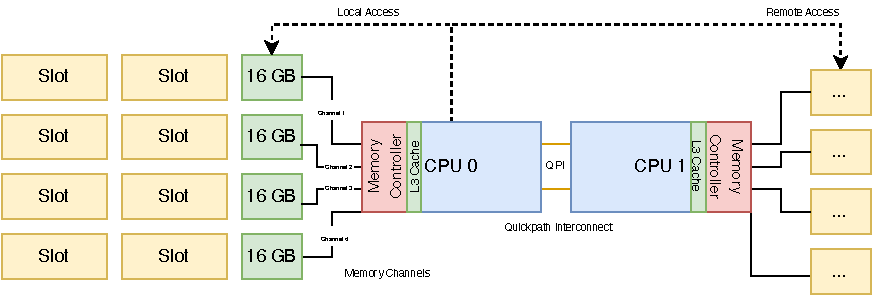
\includegraphics[scale=0.9]{fig/02/02-numa-cores.pdf}
    \caption{NUMA Core}
    \label{fig:02-numa-cores}
    \tiny
    NUMA Core Architecture showing Local and Remote Memory Access.
\end{figure}

The multiprocessor class of parallel computer represents the dominant architecture in contemporary supercomputing. Broadly defined, it consists of multiple independent processors, each with its own instruction control, interconnected through a communication network and coordinated to execute a single workload. Symmetric multiprocessors (SMPs) use a shared memory model accessible by all processors. Nonuniform memory access (NUMA) architectures extend shared-memory designs by allowing all processors to access the full memory space but with different access times depending on locality. As visualized in \ref{fig:02-numa-cores}, NUMA leverages fast local memory channels alongside slower global interconnects, enabling greater scalability than SMPs.

\subsubsection{Virtualization in HPC}
\label{sec:background_hpc_virtualization}
% TODO: Cite paper: Survey on Virtualization of HPC, M. Shao IEEE
With the ever-growing demand for HPC, hardware resources have continued to expand in scale and complexity, with increasingly intricate interconnections between system components. A central challenge lies in maximizing both performance and resource utilization. Virtualization technologies offer means to improve resource utilization in HPC environments by enabling the provisioning of resources to multiple users on the same physical machine with the goal of maximizing utilization. Depending on the abstraction layer, different virtualization technologies provide distinct benefits. Containers, which virtualize at the operating system level, offer lightweight isolation and have become widely adopted for deploying microservices \cite{9653557}.
Containers studies have shown that container performance often approaches native execution, particularly for CPU- and memory-intensive workloads, whereas VMs tend to suffer greater degradation for memory, disk, and network-intensive applications. In comparative analyses, Docker containers have demonstrated near-native efficiency for CPU and memory tasks but exhibit performance bottlenecks in certain networking and storage configurations \cite{8397647}.

\subsection{Scientific Workflows}
\label{sec:background_workflows}
%TODO: Insert Sentence between these 2 sections
% \cite{Scientific worflows: past, present and future}
\subsubsection{Scientific Workflow Management Systems}
\label{sec:background_workflows_swms}
Scientific Workflow Management Systems (SWMS's) enable the composition of complex workflow applications by connecting individual data processing tasks. Figure \ref{fig:02-swms} shows an example of an swms architecture. Tasks, often treated as black boxes, can represent arbitrary programs whose internal logic is abstracted away from the workflow system. The resulting workflows are typically modeled as directed acyclic graphs (DAGs), where channels define the dependencies between tasks: the output of one task serves as the input for one or more downstream tasks. This abstraction allows users to design scalable, reproducible workflows while managing execution complexity across diverse computational environments \cite{thamsen2025energyawareworkflowexecutionoverview}.

SWMSs'sprovide a simplified interface for specifying input and output data, enabling domain scientists to integrate and reuse existing scripts and applications without rewriting code or engaging with complex big data APIs. This abstraction lowers the entry barrier for developing and executing large-scale workflows \cite{Bader_2022}.

%SWMS architecture in general
\begin{figure}[H]
    \centering
    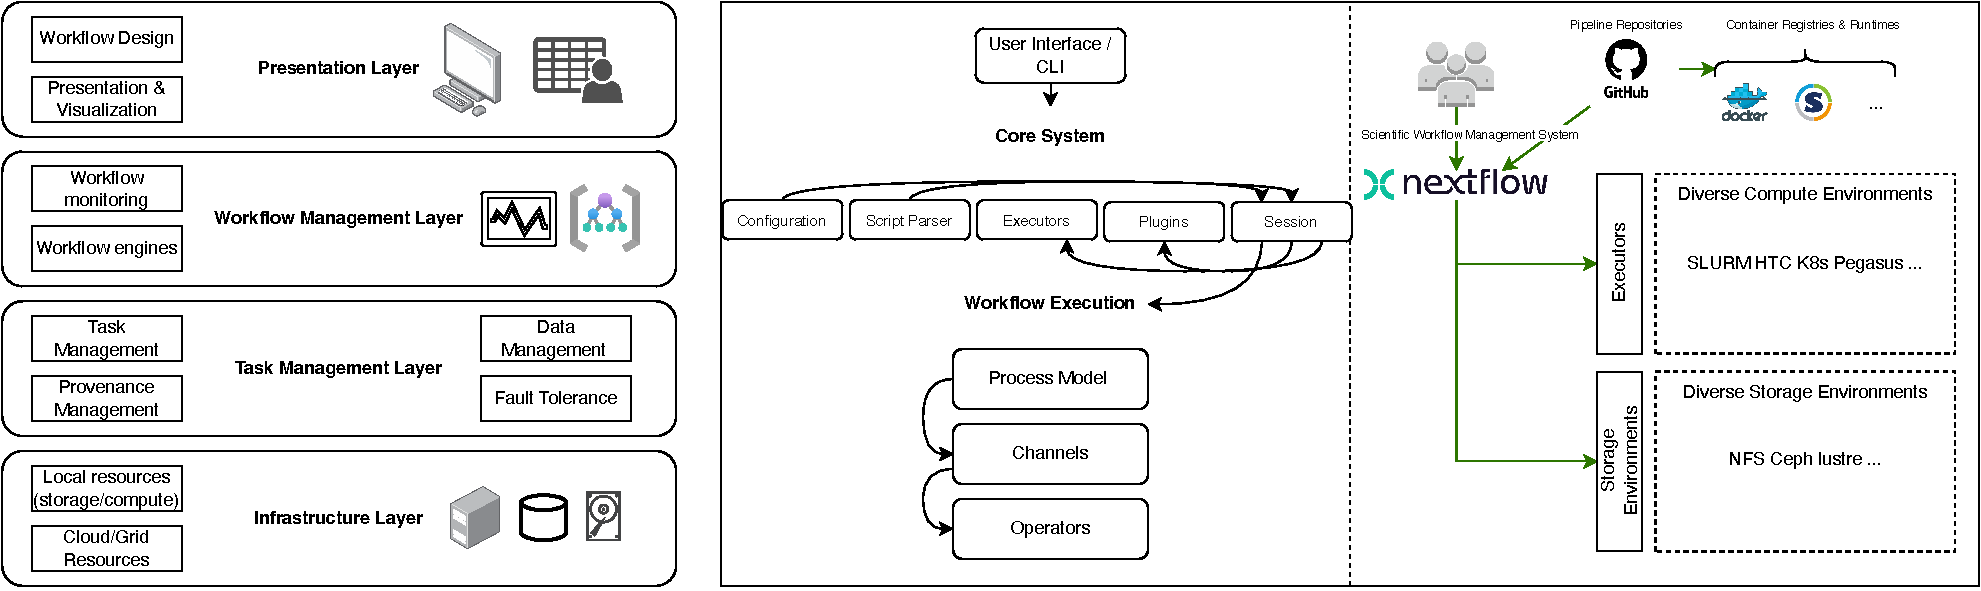
\includegraphics[scale=0.45]{fig/02/02-swms.pdf}
    \caption{Scientific Workflow Management System}
    \label{fig:02-swms}
    \tiny
    Structured Components of an exemplified Scientific Workflow Management System.
\end{figure}

\subsubsection{Scientific Workflow Tasks}
\label{sec:background_workflows_examples}
Scientific workflows are compositions of sequential and concurrent data processing tasks, whose order is determined by data interdependencies. As \ref{fig:02-workflow-task} depicts, a task is the basic data processing component of a scientific workflow, consuming data from input files or previous tasks and producing data for follow- up tasks or output files. Scientific workflows exist at different levels of abstraction: abstract, concrete, and physical. An abstract workflow models data flow as a concatenation of conceptual processing steps. Assigning actual methods to abstract tasks results in a concrete workflow. To execute a concrete workflow, input data and processing tasks have to be assigned to physical compute resources. In the context of scientific workflows, this assignment is called scheduling and task mapping and results in a physical and executable workflow \cite{Bux2013}.
Due to their complexity and scale, workflows often consist of large numbers of tasks with multiple parallel paths and are executed on clusters—collections of interconnected compute nodes managed as a single system. SWMS's submit ready-to-run tasks to cluster resource managers such as Slurm or Kubernetes, which allocate resources according to user-defined requirements like CPU cores and memory. Task communication is typically implemented via persistent cluster storage systems like Ceph, HDFS, or NFS, where intermediate data is written and read between tasks \cite{thamsen2025energyawareworkflowexecutionoverview}.

% Graphic of task 
\begin{figure}[H]
    \centering
    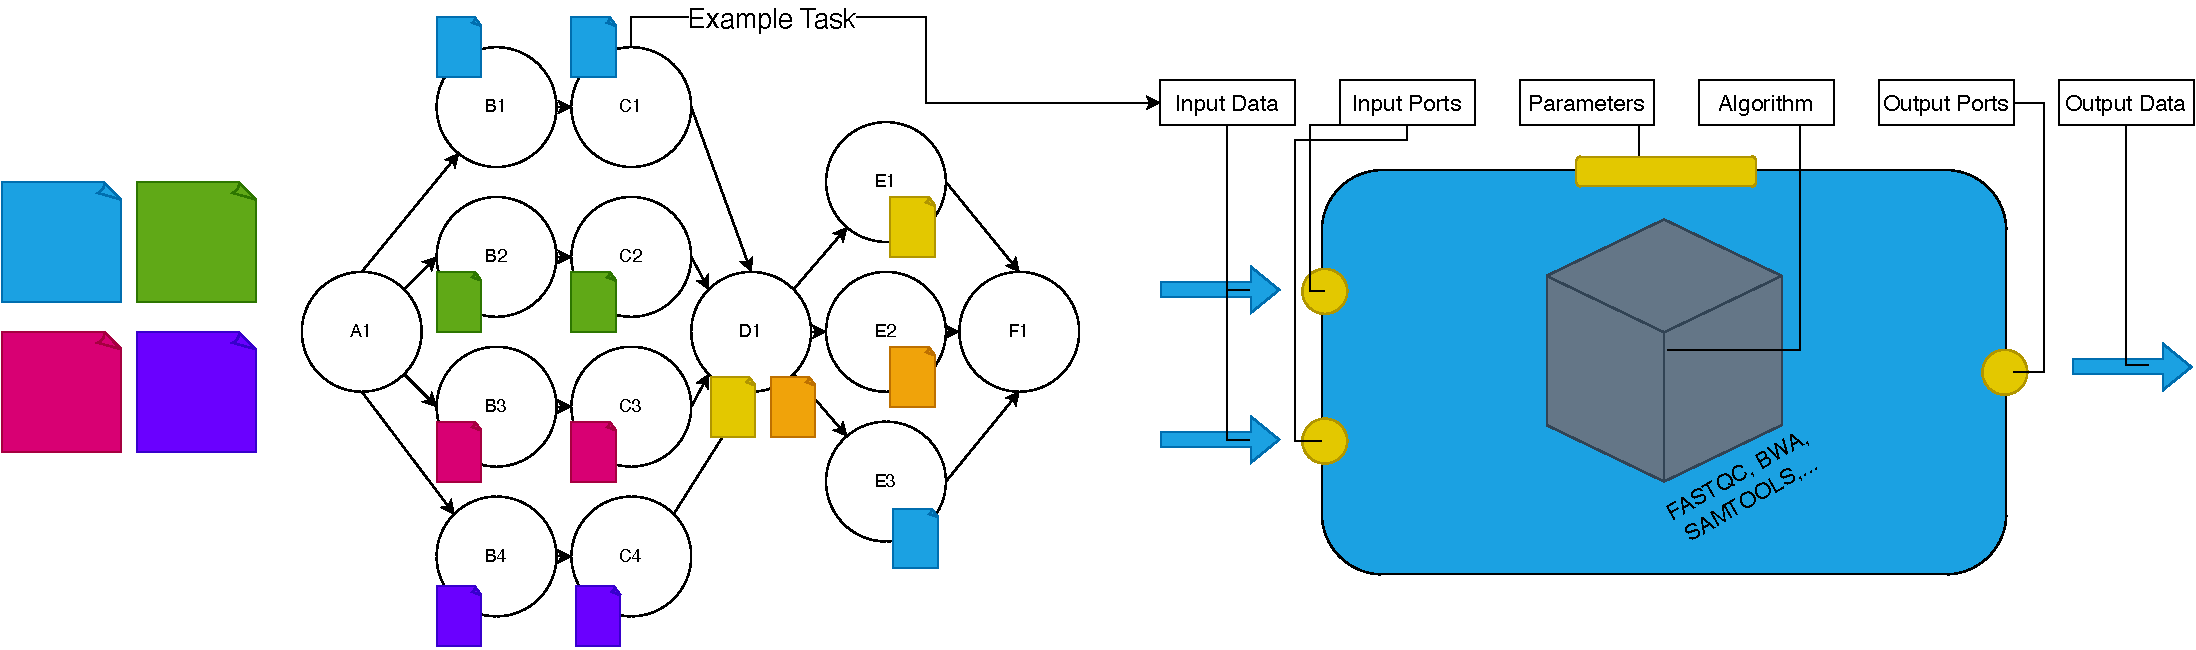
\includegraphics[scale=0.4]{fig/02/02-workflow-task.pdf}
    \caption{Workflow Task}
    \label{fig:02-workflow-task}
    \tiny
    A Scientific Workflow Task as part of a Workflow consuming input data and producing output data.
\end{figure}

\subsection{Monitoring of Scientific Workflows}
\label{sec:background_monitoring}
Performance generally helps to prevent degradation by preventable factors, for example by checking whether computation times match processor capabilities or whether communication delays align with message sizes and network bandwidth. Instrumentation of code segments can provide such insights, though even basic measurements introduce latency and overhead that may distort results or even alter execution flow. Hardware-based approaches use modern CPUs to provide dedicated performance counters for events such as instruction retirement, cache misses, or branches. These counters operate transparently, incurring virtually no overhead, though they are limited to a predefined set of measurable events \cite{STERLING201843}.

\subsubsection{Distinct Monitoring Layers}
\label{sec:background_monitoring_layers}
\paragraph{Highl-level Monitoring}
While general HPC performance monitoring tools can provide detailed insights into system resource usage, linking these measurements to higher-level abstractions such as workflow tasks remains challenging. \ref{fig:02-monitoring-layers} provides a high-level overview on the relevant monitoring layers.

% High-Level Layers
\begin{figure}[H]
    \centering
    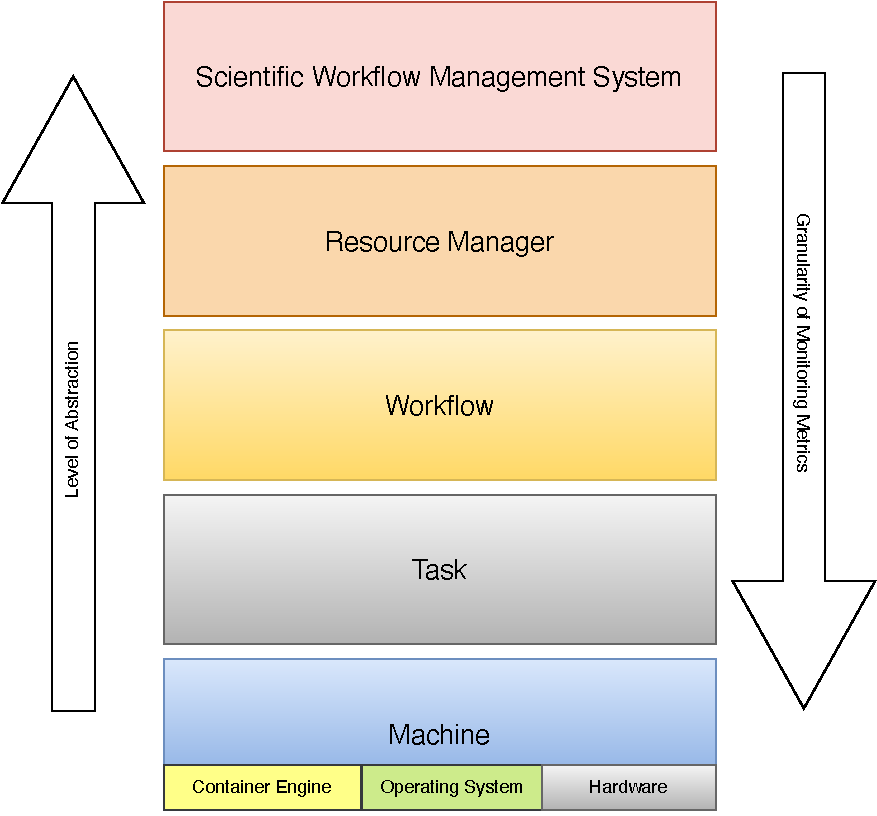
\includegraphics[scale=0.5]{fig/02/02-monitoring-layers.pdf}
    \caption{Monitoring Layers}
    \label{fig:02-monitoring-layers}
    \tiny
    Monitoring Layers in Scientific Workflows.
\end{figure}

In large-scale scientific workflows executed on distributed environments tasks may be scheduled on arbitrary nodes and may even share resources with other tasks. As a result, locally observed traces of CPU, memory, or I/O usage cannot be directly attributed to specific tasks.  Moreover, metrics natively provided by workflow management systems are often coarse-grained, capturing only summary statistics for task lifetimes. To obtain fine-grained insights into task-level behavior, additional instrumentation and mapping strategies are required to connect low-level monitoring data with workflow abstractions. To deal with this lack of information, resource usage profiles from compute nodes must be correlated with metadata such as workflow logs or job orchestrator information \cite{Witzke2024}.

To bridge this gap, \cite{Bader_2022} proposed an architectural blueprint for workflow monitoring is organized into four layers: the resource manager, the workflow, the machine, and the task layer. These layers represent logical distinctions within a scientific workflow execution environment, each focusing on a different monitoring subject and retrieving metrics from lower layers as needed. Higher layers provide increasingly abstract views, relying only on selected metrics from underlying layers while, in theory, being able to access all. Lower layers, as shown in Figure \ref{fig:02-monitoring-layers2} the resource manager level aggregates metrics like task resource consumption or available machine resources, without depending on fine-grained traces such as syscalls. The workflow layer captures metrics tied to the workflow specification, while the machine layer delivers detailed reports of node-level resource usage. At the lowest level, the task layer focuses on fine-grained task execution metrics \cite{Bader_2022}.

\paragraph{Low-level Resource Monitoring}
% TODO: Insert citation for ebpf book
Monitoring scientific workflows requires tools that can capture and relate information across different components of a computing system, since no single perspective provides sufficient detail for effective optimization. Low-level system monitors can reveal CPU, memory, or I/O usage but lack awareness of which workflow tasks generate that load, while workflow management systems expose task-level metrics that are often too coarse to identify inefficiencies. In the following, we briefly discuss tools and approaches for monitoring the low layers.
Central among low-level techniques is tracing, which captures fine-grained event-based records such as system calls, I/O operations, or network packets. The Berkeley Packet Filter (BPF) allows small programs to run directly in the kernel, making it possible to process events in real time and reduce the overhead of storing and analyzing massive trace logs. In contrast, sampling tools collect subsets of data at regular intervals to create coarse-grained performance profiles. Together with fixed hardware or software counters, tracing and sampling form the backbone of observability.
The BPF ecosystem provides several user-friendly front ends for tracing, most notably BCC (BPF Compiler Collection) and bpftrace \cite{gregg2020bpf}. Figure \ref{fig:02-ebpf-os} illustrates common monitoring targets at the OS level using eBPF.
% Monitoring targets on OS-level
\begin{figure}[H]
    \centering
    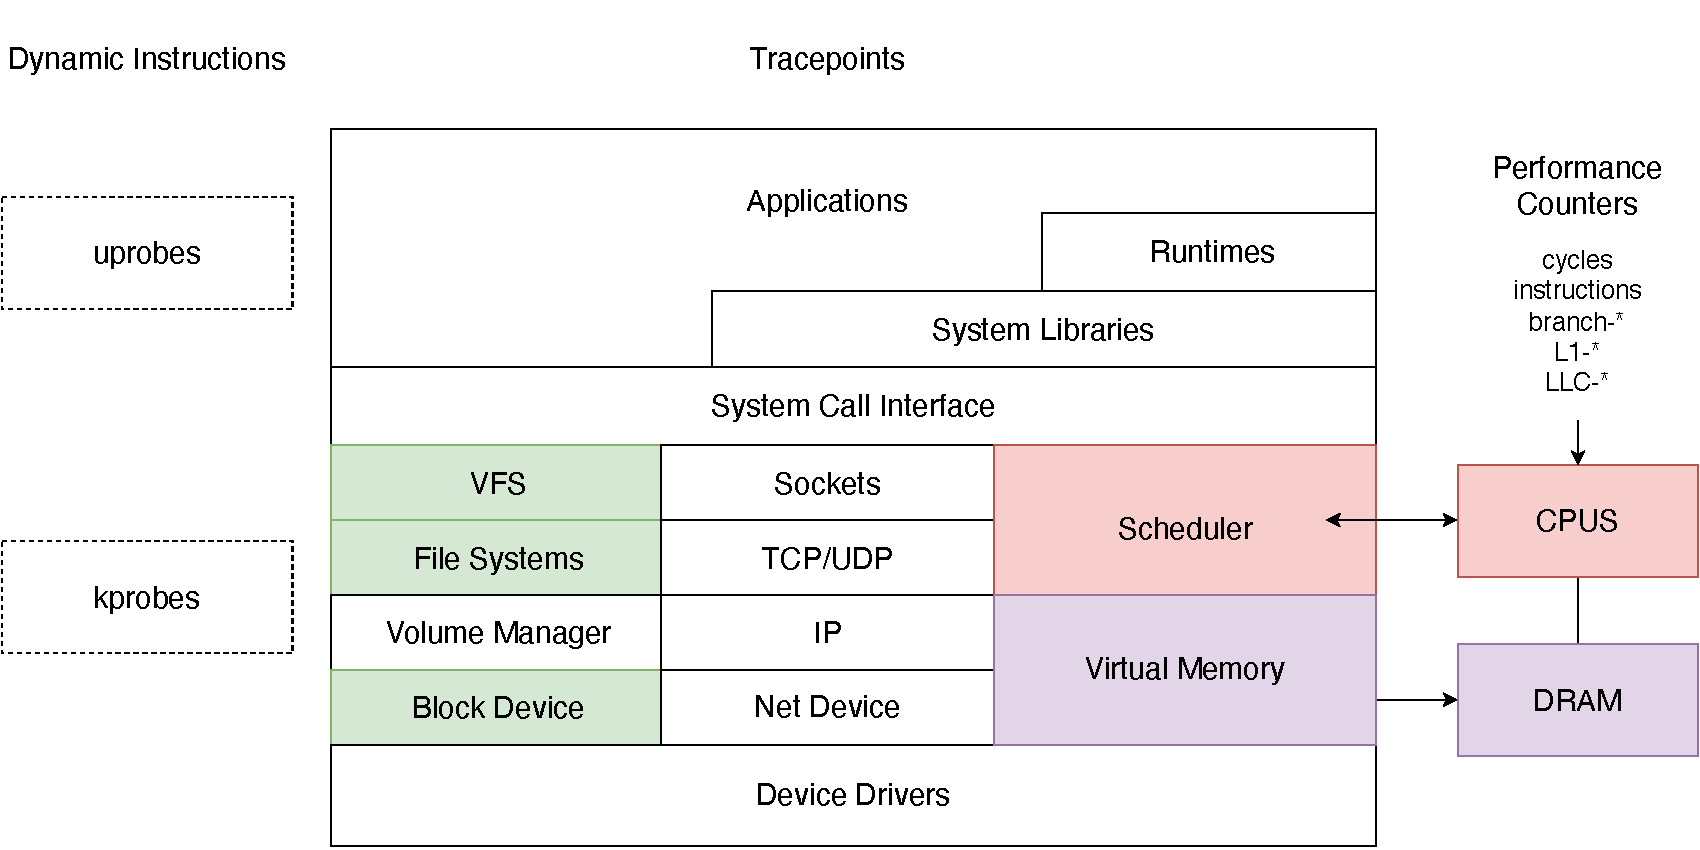
\includegraphics[scale=0.4]{fig/02/02-ebpf-os.pdf}
    \caption{Low Level Monitoring Targets.}
    \label{fig:02-ebpf-os}
    \tiny
    Low Level Monitoring Targets on the OS-Level using eBPF.
\end{figure}

Low-level performance monitoring is extensively defined by \cite{gregg2020bpf}.
CPU, memory, and disk are central components for understanding system behavior. Monitoring the CPU usage fundamentally relies on understanding how time is distributed across the execution modes and how the scheduler allocates processor resources among competing tasks. Metrics such as user time, system time, and idle time provide the basis for identifying imbalances, while additional indicators like context switches, interrupt handling, and run queue lengths reveal how efficiently the scheduler manages concurrency. Since background kernel activities and hardware interrupts can consume significant CPU cycles outside of explicit user processes, distinguishing their contribution is essential for accurate analysis \cite{gregg2020bpf}.
In close relation to CPU monitoring, effective memory performance analysis requires tracking how memory behavior influences compute efficiency. Since CPUs frequently stall waiting for data, metrics such as page faults, cache misses, and swap activity can directly translate into wasted cycles. A systematic strategy begins with checking whether the out-of-memory (OOM) killer has been invoked, as this signals critical memory pressure. From there, swap usage and I/O activity should be examined, since heavy swapping almost always leads to severe slowdowns. System-wide free memory and cache usage provide a high-level view of available resources, while per-process metrics help identify applications with excessive resident set sizes (RSS).
Following CPU and memory, file system monitoring focuses on workload behavior at the logical I/O layer and its interaction with caches and the underlying devices. Key signals include operation mix and rates such as reads, writes, opens/closes and latency distributions for I/O, and the balance of synchronous versus asynchronous writes \cite{gregg2020bpf}.

From a performance monitoring perspective, containers introduce challenges that extend beyond those encountered in traditional multi-application systems. First, cgroups may impose software limits on CPU, memory, or disk usage that can constrain workloads before physical hardware limits are reached. Detecting such throttling requires monitoring metrics that are not visible through standard process- or system-wide tools. Second, containers can suffer from resource contention in multi-tenant environments, where noisy neighbors consume disproportionate shares of the available resources, leading to unpredictable performance degradation for co-located containers.
A further complication lies in attribution. The Linux kernel itself does not assign a global container identifier. Instead, containers are represented as a combination of namespaces and cgroups, which complicates mapping low-level kernel events back to the higher-level abstraction of a specific container. While some workarounds exist—such as deriving identifiers from PID or network namespaces, or from cgroup paths—this mapping is non-trivial and runtime-specific. To address these issues, container monitoring must operate at multiple levels of abstraction. Metrics must capture both coarse-grained resource usage across cgroups and fine-grained kernel events such as scheduling latencies, memory allocation faults, and block I/O delays. At the same time, the collected data needs to be attributed correctly to the corresponding container environment in order to identify interference, diagnose bottlenecks, and evaluate orchestration policies.
Monitoring hypervisors poses challenges similar to containers but with a different focus. Since each VM runs its own kernel, guest-level monitoring tools can operate normally, but they cannot always observe the virtualization overheads introduced by the hypervisor. Key concerns include the frequency and latency of hypercalls in paravirtualized environments, the impact of hypervisor callbacks on application scheduling, and the amount of stolen CPU time—periods when a guests vCPU is preempted by the hypervisor. From the host perspective, additional events such as VM exits provide insight into how often guests trigger traps to the hypervisor, for example on I/O instructions or privileged operations, and how long these exits last. Attribution is further complicated because exit reasons vary widely across workloads and hypervisor implementations \cite{gregg2020bpf}.

\subsubsection{Monitoring Energy Consumption}
\label{sec:background_monitoring_energy}

% Overview picture
\begin{figure}[H]
    \centering
    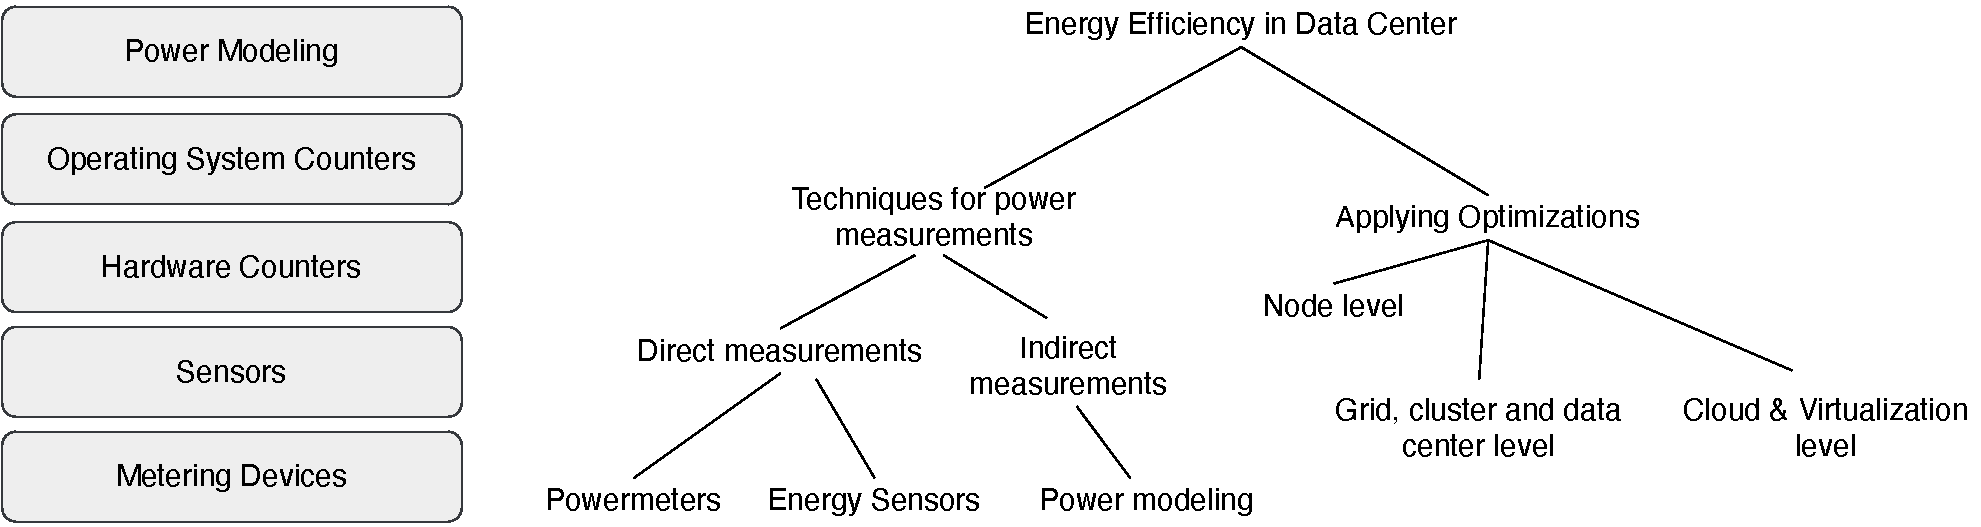
\includegraphics[scale=0.4]{fig/02/02-energy-overview.pdf}
    \caption{Power Measurements in Data Center.}
    \label{fig:02-energy-overview}
    \tiny
    Different Levels and Means of increasing energy efficiency in data centers.
\end{figure}

Conceptually shown in \ref{fig:02-energy-overview} the accurate and fine-grained energy monitoring is essential for improving the efficiency of HPC and data center systems. Traditional measurement methods, such as external power meters or chassis-level sensors, provide reliable but coarse readings at the node or rack level. These approaches are often expensive, intrusive, and insufficient for attributing power consumption to individual components or workloads. To achieve higher accuracy and temporal resolution, modern systems increasingly rely on hardware-assisted mechanisms and integrated interfaces that directly expose energy metrics from within the processor \cite{khan2018energy}.

The most widely used of these interfaces is Intel's Running Average Power Limit (RAPL), introduced with the Sandy Bridge architecture. RAPL, as visualized in \ref{fig:02-rapl}, grants direct access to cumulative energy consumption for various hardware domains, including the CPU package, cores, integrated GPU, and DRAM. In newer architectures such as Skylake, an additional PSys domain represents the overall system-on-chip energy use. Each domain reports energy data through model-specific registers (MSRs) that can be read at millisecond-level resolution. These measurements can be accessed using the Linux MSR driver, the sysfs interface, performance monitoring tools like perf, or libraries such as PAPI. RAPL's low overhead and high sampling rate have made it a standard component of modern HPC monitoring frameworks, supporting tasks from energy profiling and performance analysis to power-aware scheduling. While originally an Intel-specific technology, RAPL functionality is also available on AMD Zen architectures, although with limited support for energy domains compared to Intel implementations \cite{khan2018energy}.

% RAPL
\begin{figure}[H]
    \centering
    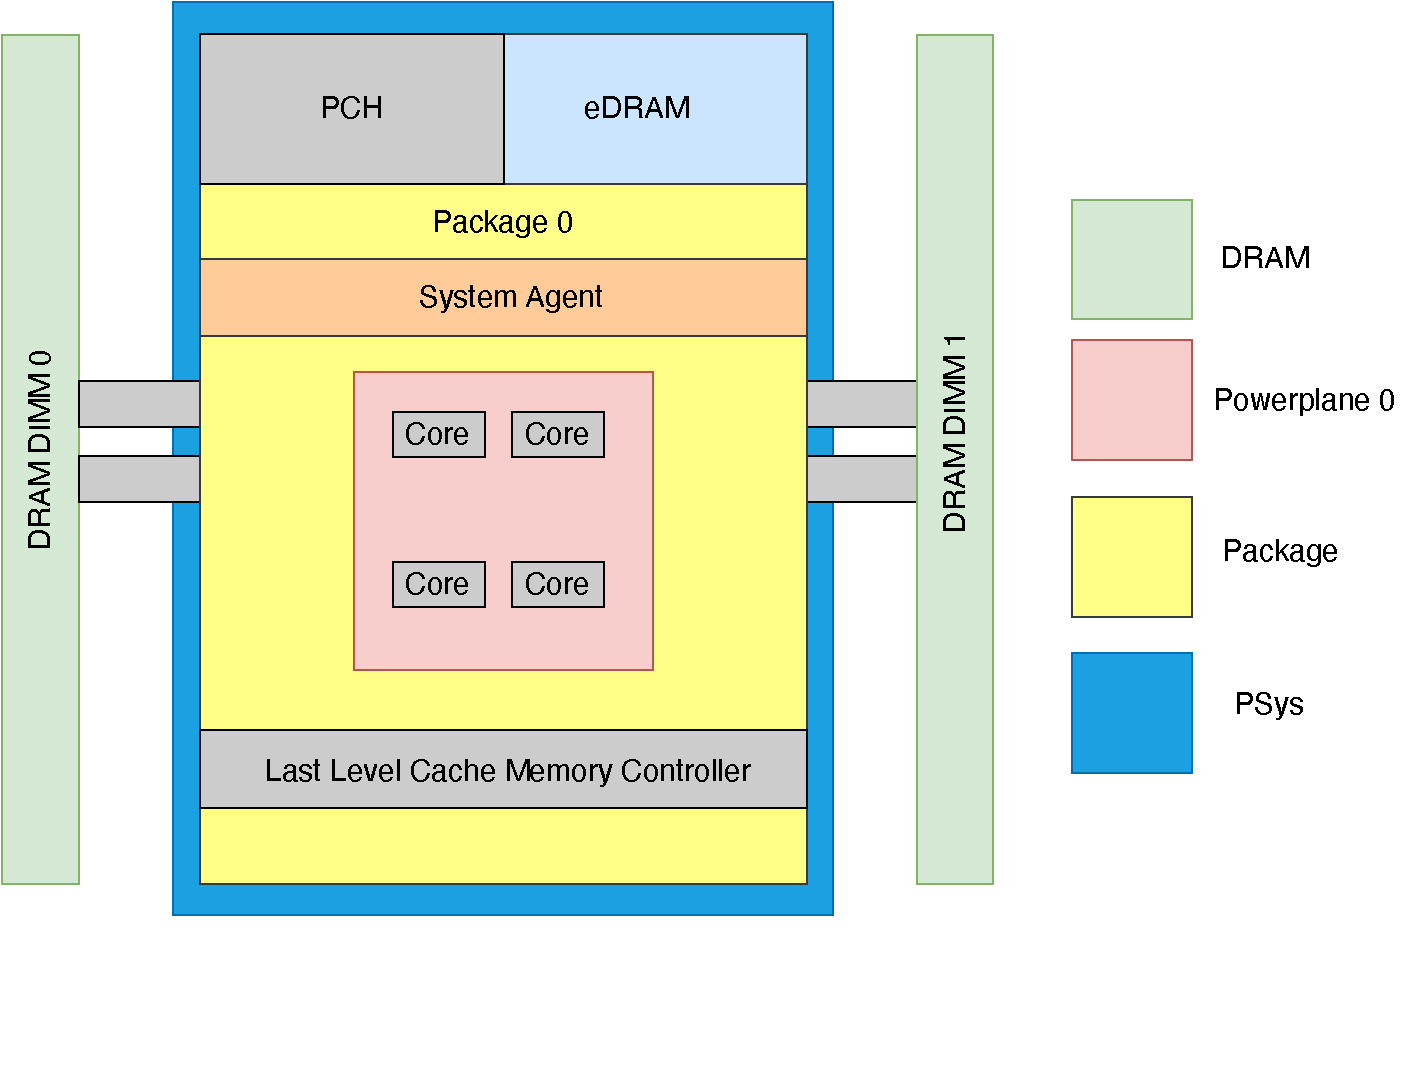
\includegraphics[scale=0.5]{fig/02/02-rapl.pdf}
    \caption{RAPL Domains}
    \label{fig:02-rapl}
    \tiny
    Overview of RAPL Energy Domains measured on a Processor.
\end{figure}

As containerization becomes standard in HPC and cloud infrastructures, energy attribution must extend from node-level to container-level granularity. Workflows composed of numerous short-lived and heterogeneous tasks require monitoring that captures both process-level activity and resource-specific energy usage. Integrating RAPL data with container-level metrics bridges this gap, enabling per-task and per-workflow energy accounting.
Tools such as DEEP-mon build on RAPL by combining kernel-level event tracing with container-level aggregation. They can attribute energy consumption to threads, processes, or containers in real time while maintaining low system overhead. Such tools extend traditional monitoring from static node metrics to dynamic, workload-aware measurements suitable for modern, containerized HPC environments. This integration of hardware-assisted measurement and software-level attribution forms the basis for energy-aware orchestration and supports the development of sustainable, performance-efficient scientific computing systems \cite{8425477}.

\subsection{The Co-location Problem}
\label{sec:background_colocation}
The problem of co-location can be traced back to classical operating system scheduling, where the core challenge lies in allocating activities to functional units in both time and space. Traditionally, scheduling in operating systems refers to assigning processes or threads to processors, but this problem appears at multiple levels of granularity, from whole programs to fine-grained instruction streams executed within superscalar architectures \cite{5702048}. On multiprocessor and multicore systems, the scheduler must not only decide when to run a task but also where, since shared caches, memory bandwidth, and execution units create interdependencies between co-located workloads. Early work in operating systems introduced co-scheduling or gang scheduling, where groups of related tasks are executed simultaneously to reduce synchronization delays, exploit data locality, and minimize contention for shared resources. These concepts are directly relevant to modern scientific workflows, where multiple interdependent tasks are often co-located on the same nodes or cores in high-performance computing environments. The performance and energy efficiency of workflows are therefore closely tied to scheduling decisions, as co-located tasks may either benefit from shared resource usage or suffer from interference, making scheduling a fundamental problem for efficient workflow execution.
Assigning each task to a separate server leads to poor energy efficiency, as servers continue to draw a substantial fraction of their peak power even under low utilization \cite{6193474} \cite{Kuity_2023}. Server consolidation thus emerges as a promising strategy, where multiple workflow tasks are mapped onto fewer servers to reduce total power consumption and resource costs. In this context, the terms consolidation and co-location can be used interchangeably, as both refer to the placement of multiple tasks onto the same physical resources with the aim of improving efficiency \cite{5644899}. However, consolidation is far from trivial: the resource usage of colocated tasks is not additive, and interference effects can significantly impact both power consumption and application performance. Furthermore, the temporal variation in workflow task demands requires runtime-aware provisioning strategies to avoid resource contention and performance degradation \cite{5644899}

\subsubsection{Impacts of Co-location on Resource Contention and Interference}
\label{sec:background_colocation_interference}

% Coloc-Problem
\begin{figure}[H]
    \centering
    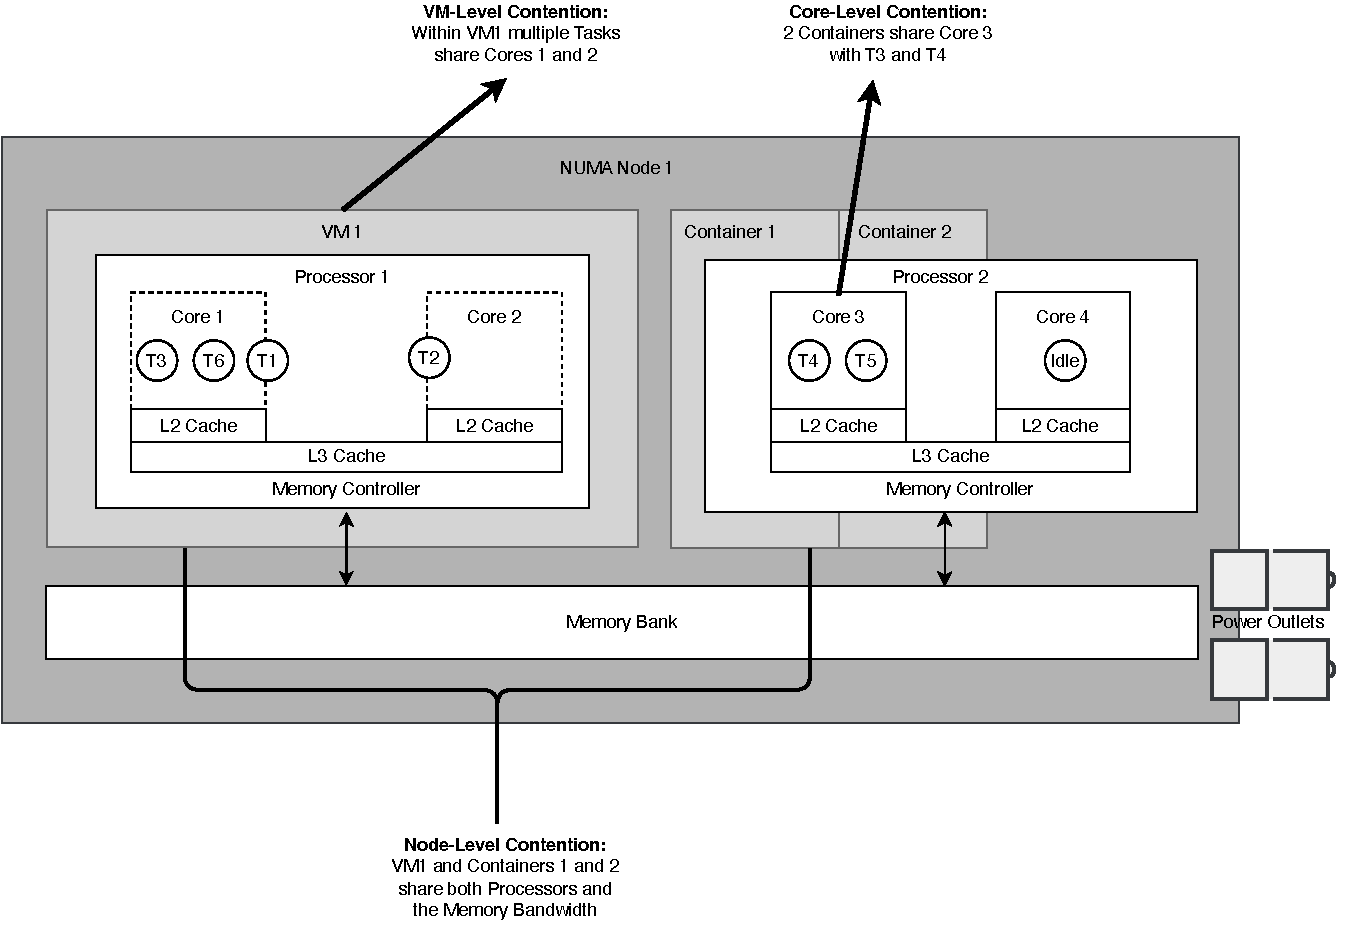
\includegraphics[scale=0.5]{fig/02/02-coloc-overview.pdf}
    \caption{The Co-location Problem.}
    \label{fig:02-coloc-overview}
    \tiny
    Different Levels of Co-location on a Compute Node.
\end{figure}

The fundamental motivation for addressing co-location in HPC and cloud environments lies in mitigating resource contention. Figure \ref{fig:02-coloc-overview} illustrates three possible levels of contention that can occur on a single compute node. Tasks may share CPU cores within a virtual machine, multiple containers can be pinned to the same core, and even the placement of virtual machines and containers themselves introduces additional layers of co-location effects that influence overall performance and energy efficiency. When processes execute on different cores of the same server, they inevitably share hardware resources \cite{Blagodurov_2010} \cite{7349920}. Modern multi-core architectures share on-chip structures such as last-level caches, memory controllers, and interconnects, as well as off-chip memory bandwidth, creating significant opportunities for contention when multiple applications run concurrently. This contention can result in severe performance degradation, making it critical to understand and predict the impact of co-location on application efficiency \cite{Blagodurov_2012}. As a result this interference slows down execution compared to scenarios where tasks have exclusive access to these resources. In extreme cases, memory traffic contention has been shown to cause slowdowns, where execution times more than double, making sequential execution more efficient than poorly chosen co-schedules. For large-scale systems hosting thousands of tasks, this contention complicates job scheduling, as schedulers must avoid placing workloads that compete heavily for the same resources. Without accurate estimates of resource usage or slowdown potential, scheduling decisions risk becoming guesswork, reducing overall efficiency. Importantly, poor scheduling is not limited to high-resource applications: even pairing computationally bound tasks that do not interfere can be suboptimal if it prevents beneficial co-scheduling with memory-bound applications. This highlights that effective co-location must avoid both high-contention pairings and missed opportunities for complementary workload placement \cite{inproceedings} \cite{10.1007/978-3-031-48803-0_31}.

\subsubsection{Shared Aspects and Distinctions from Scheduling and Task Mapping}
\label{sec:background_colocation_scheduling}
Co-location differs fundamentally from scheduling and task mapping, even though all three can aim at improving performance and energy efficiency in workflow execution. Scheduling determines when each task runs, while mapping decides where each task is placed \cite{9284517} \cite{Merkel_2010}. In contrast, co-location focuses on how tasks interact when they are executed simultaneously on shared resources \cite{9499521} \cite{9112926} \cite{Dauwe_2016}.
Scheduling and mapping operate primarily at the planning level—deciding task order and resource assignment to optimize overall throughput, energy use, or completion time \cite{Choudhary_2022}. Co-location, however, concerns the execution-level effects that arise once multiple tasks occupy the same physical resources. It addresses the contention for shared hardware components such as caches, memory bandwidth, interconnects, and I/O subsystems.
While scheduling seeks to allocate time and space efficiently, co-location must manage interference that emerges during concurrent execution. Poor co-location decisions can negate the benefits of an otherwise optimal schedule by causing resource contention, latency, or performance degradation. Therefore, co-location is not an extension of scheduling but a complementary consideration that governs how shared resource usage affects the actual efficiency and energy behavior of scheduled tasks \cite{5644899}.

\subsection{Machine Learning Techniques applied in HPC}
\label{sec:background_ml}

\subsubsection{Intelligent Resource Management}
\label{sec:background_ml_resourcemanagement}
When executing scientific workflows on large-scale computing infrastructures, researchers are required to define task-level resource limits, such as execution time or memory usage, to ensure that tasks complete successfully under the control of cluster resource managers. However, these estimates are often inaccurate, as resource demands can vary significantly across workflow tasks and between different input datasets, leading either to task failures when limits are underestimated or to inefficient overprovisioning when limits are set too conservatively \cite{BADER2024171}. Overprovisioning, while preventing failures, reduces cluster parallelism and throughput, as excess resources are reserved but left unused, while incorrect runtime estimates can distort scheduling decisions and degrade overall system efficiency. To address this, recent research has explored workflow task performance prediction as a means to automate the estimation of runtime, memory, and other resource needs. Machine learning plays a central role in these efforts, with approaches ranging from offline models trained on historical execution data, to online models that adapt dynamically during workflow execution, to profiling-based methods applied before execution \cite{Hou_2022} \cite{Borghesi_2016} \cite{10061770}. Performance prediction models can integrate into both workflow management systems and resource managers, enabling more informed scheduling, efficient resource utilization, and improved energy- and cost-aware computing \cite{bader2025predictingperformancescientificworkflows}  \cite{ZACARIAS2021125}.

\subsubsection{Utilized Machine Learning Models in this Thesis}
\label{sec:background_ml_algorithms}

\paragraph{Ordinary Least Squares and Extensions}
\label{sec:background_ml_lr}
% TODO: add citation for sklearn documentation.
\myparagraph{Kernel Ridge Regression}
Kernel Ridge Regression (KRR) builds on ordinary least squares (OLS) regression. OLS learns a linear relationship between input variables and a target variable by minimizing the squared difference between predictions and actual values. Ridge regression extends OLS by adding a penalty to the model coefficients, which controls overfitting and improves stability when features are correlated or data are noisy.
KRR further extends ridge regression by applying the kernel trick. Instead of fitting a linear model directly in the input space, KRR implicitly maps the data into a high-dimensional feature space defined by a kernel function, such as a Gaussian or polynomial kernel. A linear model is then learned in this new space, which corresponds to a nonlinear function in the original space when a nonlinear kernel is used.
Overall, Kernel Ridge Regression combines the simplicity and stability of ridge regression with the flexibility of kernel-based learning to model nonlinear relationships effectively \href{https://scikit-learn.org/stable/modules/linear_model.html}{Scikit-learn documentation}.

\myparagraph{Kernel Canonical Correlation Analysis}
\label{sec:background_ml_kcca}
Kernel Canonical Correlation Analysis (KCCA) is a statistical technique designed to identify and maximize correlations between two sets of variables. Unlike Principal Component Analysis, which focuses on variance within a single dataset, CCA aims to find linear projections of two datasets such that their correlation is maximized. The result is a set of canonical variables that capture the strongest relationships between the two domains. KCCA extends this idea by applying kernel methods, allowing the detection of nonlinear relationships. In KCCA, the data are implicitly mapped into high-dimensional feature spaces through kernel functions, and correlations are then maximized in that transformed space. This enables KCCA to capture more complex dependencies than linear CCA, making it particularly powerful in settings where relationships between datasets are not strictly linear \cite{1202783} \cite{5644899} \href{https://cca-zoo.readthedocs.io/en/stable/modules/generated/cca_zoo.nonparametric.KCCA.html#cca_zoo.nonparametric.KCCA}{CCA-Zoo documentation on nonparametric KCCA}.

\myparagraph{Random Forest Regression}
\label{sec:background_ml_rfr}
% Add citation from sklearn documentation
% Figure
\begin{figure}[H]
    \centering
    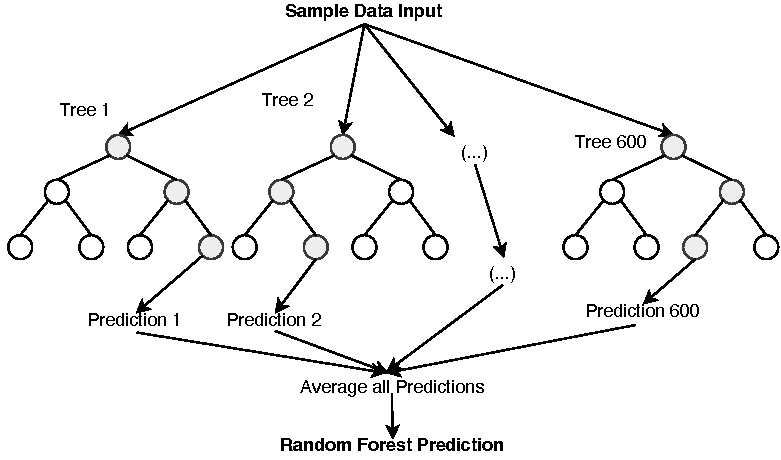
\includegraphics[scale=0.7]{fig/02/02-rf.pdf}
    \caption{Random Forest Procedure}
    \label{fig:02-rf}
    \tiny
    The iterative process of building a Random Forest for prediction.
\end{figure}

Visualized in \ref{fig:02-rf} a Random Forest Regressor is an ensemble learning method that builds multiple decision tree regressors on random subsets of the training data and combines their predictions through averaging. This approach reduces variance compared to a single decision tree, improving predictive accuracy and robustness against overfitting. Each tree is constructed using the best possible splits of the features, while the randomness introduced through bootstrap sampling and feature selection ensures diversity among the trees. An additional advantage is the native handling of missing values. During training, the algorithm learns how to direct samples with missing entries at each split, and during prediction, such samples are consistently routed based on the learned strategy. This makes Random Forest a flexible and powerful method for regression tasks with heterogeneous and potentially incomplete data \cite{Breiman2001RandomF} \href{https://scikit-learn.org/stable/modules/generated/sklearn.ensemble.RandomForestRegressor.html}{Scikit-learn documentation on RandomForestRegressor}.

\myparagraph{Agglomerative Clustering}
\label{sec:background_ml_ac}

% Figure
\begin{figure}[H]
    \centering
    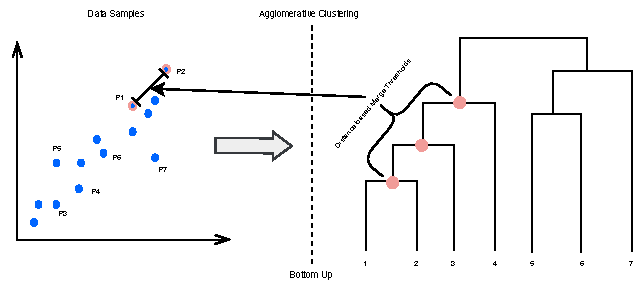
\includegraphics{fig/02/02-clustering.pdf}
    \caption{Agglomerative Clustering Procedure}
    \label{fig:02-clustering}
    \tiny
    Agglomerative Clustering applied on a distribution using a distance criterion.
\end{figure}

Agglomerative clustering, also called hierarchical clustering is a family of algorithms that group data into nested clusters, represented as a tree-like structure called a dendrogram. Figure \ref{fig:02-clustering} provides an overview on the process from raw data to clusters. In this hierarchy, each data point starts as its own cluster, and clusters are successively merged until all points form a single cluster. The commonly used agglomerative approach follows this bottom-up process, with the merging strategy determined by a chosen linkage criterion. Ward linkage minimizes the total variance within clusters, producing compact and homogeneous groups, while complete linkage minimizes the maximum distance between points in different clusters, emphasizing tight cluster boundaries. Average linkage instead considers the mean distance across all points between clusters, and single linkage focuses on the minimum distance, often resulting in elongated or chain-like clusters. Although flexible, agglomerative clustering can be computationally expensive without additional constraints, as it evaluates all possible merges at each step \href{https://scikit-learn.org/stable/modules/clustering.html#hierarchical-clustering}{Scikit-learn documentation on hierarchical clustering}.

\subsection{Research-oriented Simulation of Distributed Computing}
\label{sec:background_simulation}

WRENCH was introduced as a simulation framework that provides accurate, scalable, and expressive experimentation capabilities. Figure \ref{fig:02-wrench} conceptualizes WRENCH's framework architecture. Building on SimGrid, WRENCH abstracts away the complexity of simulating distributed infrastructures while preserving realistic models of computation, communication, storage, and failures. It provides a Developer API for implementing simulated WMSs and a User API for creating simulators that run workflows on simulated platforms with minimal code. Through these abstractions, WRENCH allows researchers to test scheduling, resource allocation, and fault-tolerance strategies at scale without the prohibitive cost of real-world deployments. Importantly, WRENCH supports a wide range of distributed computing scenarios, including cloud, cluster, and HPC environments, enabling reproducible and comparative studies of WMS design choices \cite{wrench}.

% Figure
\begin{figure}[H]
    \centering
    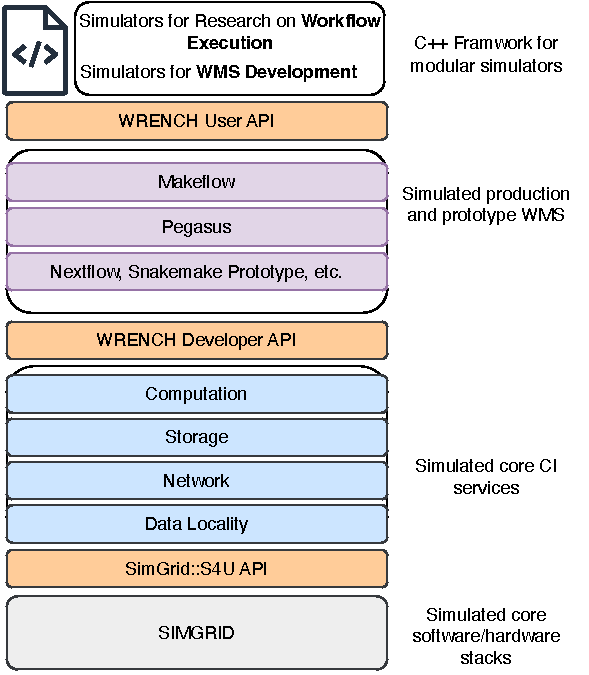
\includegraphics[scale=0.7]{fig/02/02-wrench.pdf}
    \caption{WRENCH}
    \label{fig:02-wrench}
    \tiny
    The WRENCH framework's layered architecture.
\end{figure}





